\documentclass[cjk,dvipdfmx,12pt,%
hyperref={bookmarks=true,bookmarksnumbered=true,bookmarksopen=false,%
colorlinks=false,%
pdftitle={第40回 関西Debian勉強会},%
pdfauthor={倉敷・のがた・佐々木},%
%pdfinstitute={関西Debian勉強会},%
pdfsubject={資料},%
}]{beamer}

\title{第40回 関西Debian勉強会}
\subtitle{{\scriptsize 資料}}
\author[佐々木 洋平]{{\large\bf 倉敷・のがた・佐々木}}
\institute[Debian JP]{{\normalsize\tt 関西Debian勉強会}}
\date{{\small 2010 年 10 月 24 日}}

%\usepackage{amsmath}
%\usepackage{amssymb}
\usepackage{graphicx}
\usepackage{moreverb}
\usepackage[varg]{txfonts}
\AtBeginDvi{\special{pdf:tounicode EUC-UCS2}}
\usetheme{Kyoto}
\def\museincludegraphics{%
  \begingroup
  \catcode`\|=0
  \catcode`\\=12
  \catcode`\#=12
  \includegraphics[width=0.9\textwidth]}
%\renewcommand{\familydefault}{\sfdefault}
%\renewcommand{\kanjifamilydefault}{\sfdefault}
\begin{document}
\settitleslide
\begin{frame}
\titlepage
\end{frame}
\setdefaultslide

\begin{frame}[fragile]
\frametitle{Agenda}

\tableofcontents

\end{frame}

\section{最近の Debian 関係のイベント}


\takahashi[40]{最近のDebian\\関係のイベント}
 

\begin{frame}[fragile]
\frametitle{第 39 回関西 Debian 勉強会}

9月26日に 京都高度技術研究所(ASTEM) で開催.

\begin{block}{タイル型ウィンドウマネージャ対決}
\begin{itemize}
\item タイル型ウィンドウマネージャの入門 \& dwm の解説  \\ by 山田洋平さん
\item xmonad の解説 by 倉敷悟さん
\item awesome の解説 by 山下尊也さん
\end{itemize}
\end{block}

\dots{}その後ビアバッシュ\dots{}

\end{frame}

\begin{frame}[fragile]
\frametitle{第 39 回関西 Debian 勉強会\dots{}続き}


\begin{figure}[h]
    \centering
    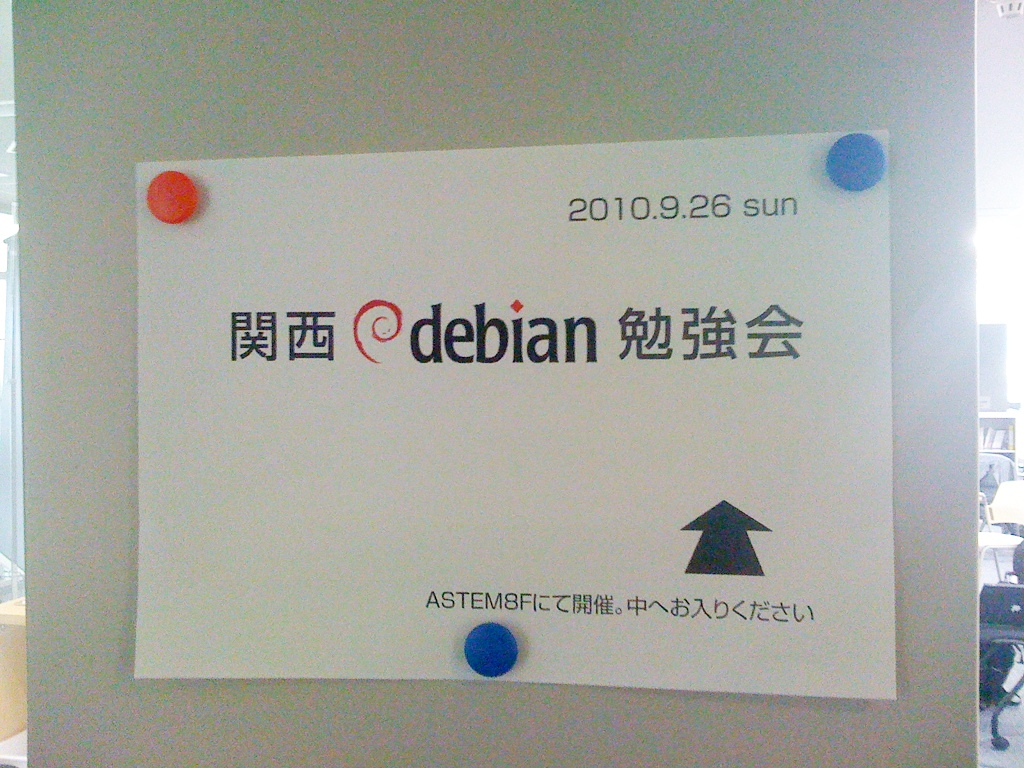
\includegraphics[width=0.35\textwidth]{image201010/kansaidebian1.jpg}
    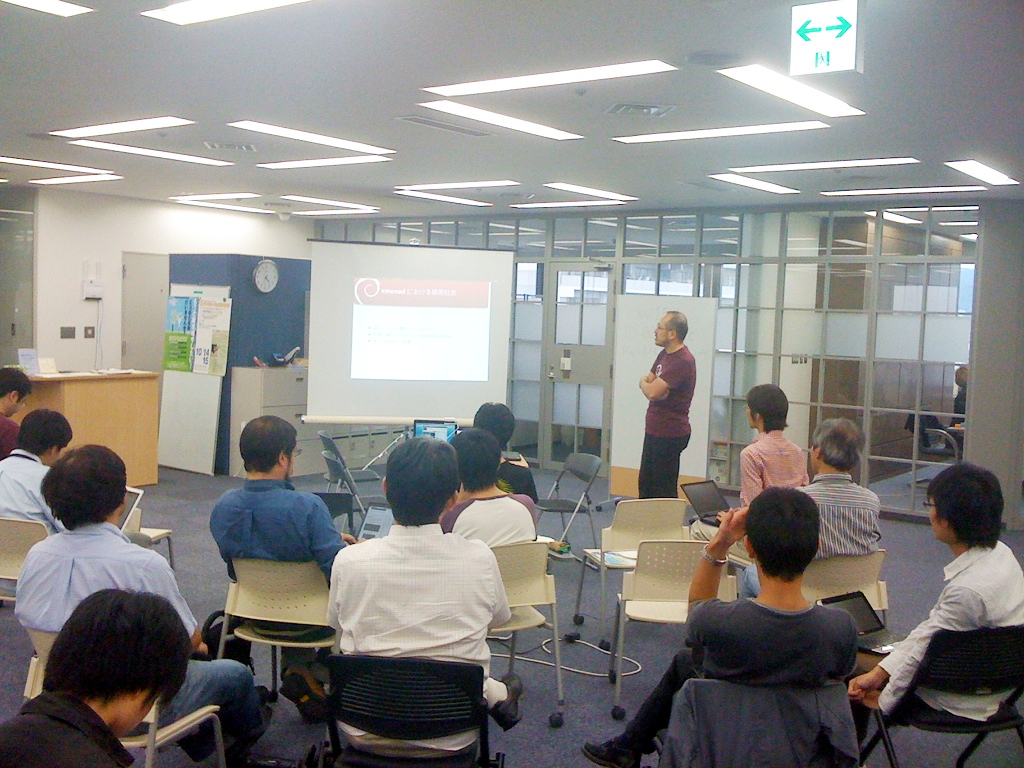
\includegraphics[width=0.35\textwidth]{image201010/kansaidebian2.jpg}
    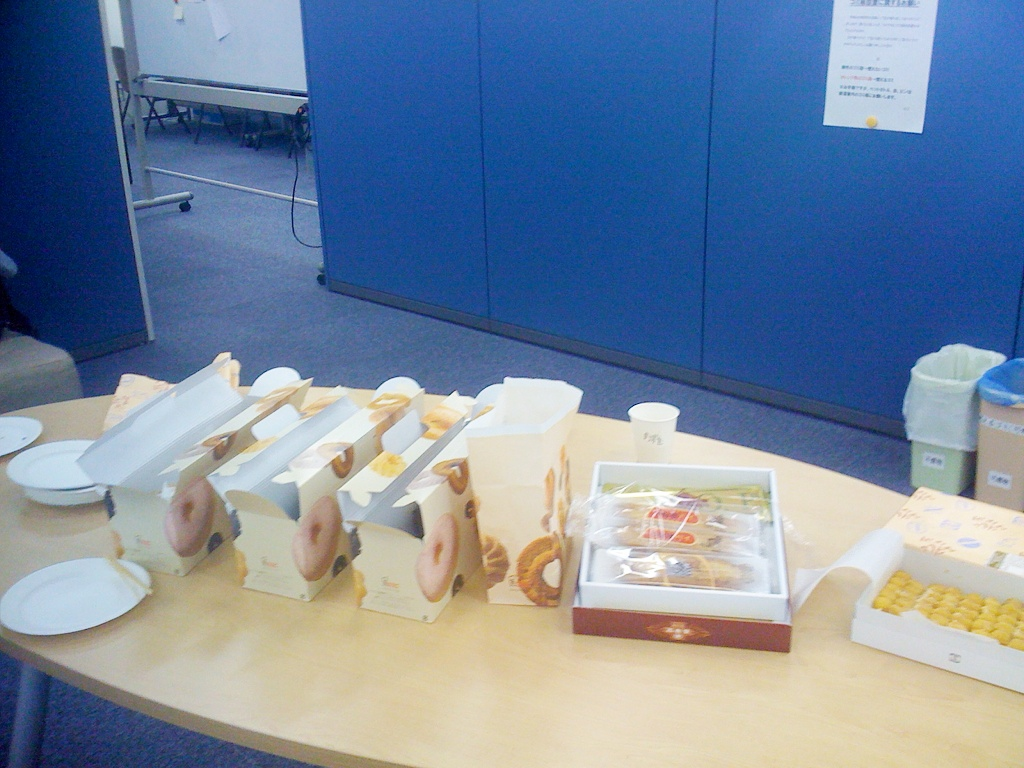
\includegraphics[width=0.35\textwidth]{image201010/kansaidebian3.jpg}
\end{figure}


\end{frame}

\begin{frame}[fragile]
\frametitle{日本 OSS 貢献者賞,OSS 奨励賞}

\begin{itemize}
\item 2010 年度の受賞者発表, Debian JP Project より

\begin{itemize}
\item OSS 貢献者賞: 武藤 健志さん
\item OSS 奨励賞: 岩松 信洋さん
\end{itemize}
\item 来週 10/28 に受賞講演があります.
\end{itemize}

\end{frame}

\begin{frame}[fragile]
\frametitle{第 69 回東京エリア Debian 勉強会}

\begin{itemize}
\item 10 月 16 日に開催
\item OSC Hokkaido, Debconf 10 の報告, 「俺の Debian な一日」

\begin{itemize}
\item 「俺の Debian な一日」はオモシロイ. 必読!
\end{itemize}
\item Debian Miniconf in Japan に関するブレスト
\end{itemize}

\end{frame}



\section{事前課題発表}


\takahashi[50]{事前課題}


\begin{frame}[fragile]
\frametitle{今回の事前課題}


\begin{block}{今回は initramfs/Debian Live のお話, ということで}
         レスキュー用途とインストール用途を除く、
        ライブシステムを使用する状況や用途を教えて(または考えて)ください。
\end{block}


\end{frame}


\takahashi[50]{事前課題\\発表}




\begin{frame}[fragile]
\frametitle{ Ipv6waterstar }


現在, インストールしている Debian システムの環境を変えずに別のシステム環境を試したい時など.


\end{frame}



\begin{frame}[fragile]
\frametitle{ dictoss (杉本  典充) }


    \begin{itemize}
          \item 公共スペースに設置するパソコンのブートディスクとして使用する.
         \\
        そうすると OS やアプリの設定を勝手に変えられても再起動すれば直るため, OS の修復の手間が省ける.
        (ネットワークブートという手もあるが, ライブシステムはスタンドアロンで起動可能な分, 敷居が低い)
\end{itemize}


\end{frame}



\begin{frame}[fragile]
\frametitle{ 山田 洋平 }


昔 1FD Linux で HDD の載ってない古い PC を動かして, 起動後はディスクレスだから静穏とか言ってました. ルータとかに使ってました. そういうのとか.
あるいはいろんな環境をとっかえひっかえ試すとか. ソフトのテスト環境としてとか. (仮想化でもいいのだけど)


\end{frame}



\begin{frame}[fragile]
\frametitle{ かわだてつたろう }


    \begin{itemize}
          \item 借り物の PC や不特定の人が使う PC で自分好みの環境を使うため
          \item 複数の人に同じ環境, アプリケーションを使ってもらいたい場合.
        「第 37 回関西 Debian 勉強会@OSC2010 Kyoto 」とか OSM で JOSM の使い方講習をするといったような用途
    \end{itemize}



\end{frame}



\begin{frame}[fragile]
\frametitle{ 八津尾  雄介 }

    \begin{enumerate}
          \item パーティションが一杯になって拡張が必要なとき.
        (これもレスキューですか?)
          \item 自分の環境を持ち歩きたいとき.
    \end{enumerate}


\end{frame}



\begin{frame}[fragile]
\frametitle{@tetsu\textunderscore{}koba }


例えば, 同僚が「今日は一日外出するのでデスクトップ PC は使わない」とする.
その PC をライブ CD で起動して distcc のサーバを動かす.
ビルドする時にその PC の CPU パワーを借りて分散コンパイルする.

これがお手軽にできるセットがあったら使ってみたい.


\end{frame}











\begin{frame}[fragile]
\frametitle{ 佐藤誠 }


    \begin{itemize}
          \item データ削除 \\
        wipe-out のように, それに特化したライブシステムもあります.
          \item アドホックなシステム構築 \\
常時接続の切れたとき, 即席のルータを構築して凌いだことがあります.
このような時は, ユーザデータや余計な設定のないライブシステムが便利だと思います.
Knoppix Hacks には, MySQL データベースの即席構築例が載っていました
(まあ, このあたりもレスキュー用途に入りそうですが)
    \end{itemize}


\end{frame}



\begin{frame}[fragile]
\frametitle{ 西山和広 }


    uuuu という勉強会
    で YouTube の講義ビデオを再生するのに, ノート PC の内蔵 HDD が不調のため, netboot のライブ環境を使っています.
    プログラムのテスト環境にも使いたいのですが, データベースを使うものの場合, メモリ不足で厳しいようです.

        uuuu: http://www.cuzic.com/undefineduniversityuponustream


\end{frame}



\begin{frame}[fragile]
\frametitle{ 'まさ'こと'甲斐正三'です }


以下の用途は実施したことはありませんが, 実施可能性ありと
思われる場面を想定したものです.
\begin{itemize}
      \item 教育用途 (案) \\
    セミナーのハンズオンを行うとき, 受講者全員に共通な環境を提供する.
      \item 新規システム等の評価検討用 (案) \\
    新規システムや新規ソフトウエアを事前評価,
    検討する際に使用する.
    例として,
    \begin{itemize}
          \item ある PC に Debian をインストールできそうかどうかをその PC 自体を使って Live CD で起動してみる.
    \end{itemize}
\end{itemize}


\end{frame}



\begin{frame}[fragile]
\frametitle{ takuya.1st }


シンクライアントとか?

みんなが帰ったとの PC にライブシステム突っ込んで分散処理を作るとか?

もちろん, ソフトウェアのデモ用にも使えますよね.
KOF のような展示会用に PC を毎回作らなくても CD 用意して持って行けば OK とか



\end{frame}



\begin{frame}[fragile]
\frametitle{ lurdan }


最近は起動も速いみたいだし, なんらかのクラウドストレージを HOME として組み込んだら, シンプルなクライアントとしては充分だったりするんじゃないかと妄想.


\end{frame}



\begin{frame}[fragile]
\frametitle{ 佐々木洋平 }


以前, ハンズオン形式の実習/ 教育機関での計算機演習などで, 受講者の環境を揃えるために使用しました (その時には, CentOS と Debian の dual boot な環境が必要で, DebianLive のエキスパートであるのがたさんに助けて頂きました).


\end{frame}



\begin{frame}[fragile]
\frametitle{ のがたじゅん }


古くなった PC にライブシステムを組み込みメンテナンスフリーなシステムを作りました. ほかにはネットワークからブートするライブシステムで面白いことできないかなーと思案中.


\end{frame}



\takahashi[50]{そんな\\こんなで}
\takahashi[120]{次}



\section{initramfs について by 西山和広さん}


\takahashi[50]{initramfs について by 西山和広さん}
\takahashi[50]{そんな\\こんなで}
\takahashi[120]{次}



\section{最近の Debian Live の動向 by のがたじゅん}


\takahashi[50]{最近の Debian Live の動向 by のがたじゅん}
\takahashi[50]{そんな\\こんなで}
\takahashi[120]{次}


\begin{frame}[fragile]
\frametitle{今後の予定}

\begin{itemize}
\item 関西オープンソース2010 + 関西コミュニティ大決戦

\begin{itemize}
\item \url{http://k-of.jp/2010/index.html}
\end{itemize}
\item ブース内容これから決める Yo!!
\item セッションは以下
\end{itemize}

\begin{block}{%
でびあん らんだむとぴっくす%
{\tiny{〜 Squeezeマダァー?(・∀・ )っ/凵⌒☆チンチン 〜}}}
11/06 13:00〜 (50 min), 9F セミナールーム2
\end{block}
\begin{block}{GPG キーサインパーティ}
11/06 17:00〜 (50 min), 9F セミナールーム3
\end{block}


\end{frame}

\begin{frame}[fragile]
\frametitle{今後の予定(2)}


\begin{block}{第 42 回関西 Debian 勉強会}
\begin{itemize}
  \item 日時: 12 月 26 日
  \item 会場: 大阪: 福島区民センター
  \item 内容: 未定
  \begin{itemize}
    \item 今年一年をふりかえる? 年度末の方が良い?
    \item リリースに向けて?
    \item 忘年会(これは必須でしょう)
  \end{itemize}
\end{itemize}
\end{block}



\end{frame}



\takahashi[50]{ }


\end{document}
%%% Local Variables: 
%%% mode: japanese-latex
%%% TeX-master: t
%%% End: 
